\newpage

\begin{figure}[h]
	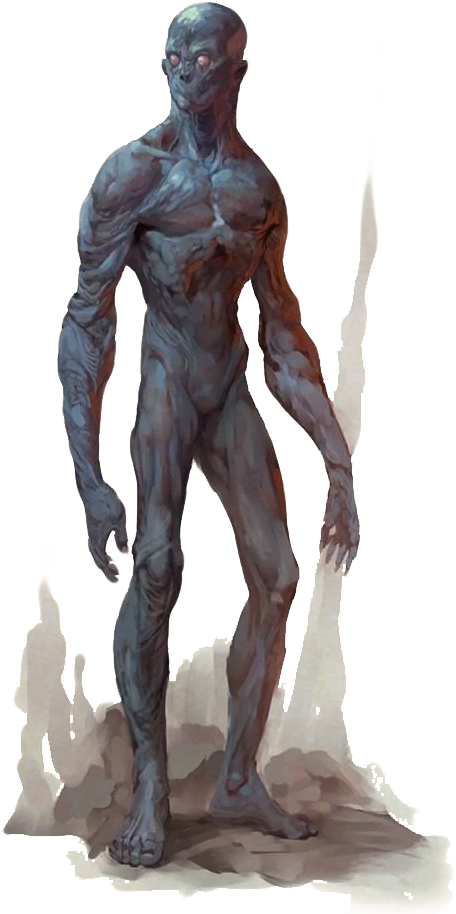
\includegraphics[width=\columnwidth-\columnsep]{doppelganger}
\end{figure}
{\vspace{-3em}}

\section{Doppelganger}
\par{Many cultures around the world feature terrifying stories of monsters that steal the souls of mortals to take on their appearance and destroy their lives. They whisper of the frightening, alien horror of such beings, and the pain they inflict in their wake.}
\par{The truth is much less fantastic: these legendary shapeshifters are actually doppelgangers. Doppelgangers are, by and large, lazy hedonists who harm others more out of self-centered greed than deliberate malice. They are usually created when doppelgangers, who can’t be bothered to put in the effort of raising their own children, seduce and impregnate women whose children grow up to, around adolescence, become doppelgangers themselves.}
\par{Still, like all mortals, doppelgangers are capable of making their own moral choices, and occasionally one rouses itself to do more with its life than an endless sequence of cons and robberies. \cite{d-hb}}

\subparagraph{Stealing Secrets}
{A doppelganger’s adopted form allows it to blend into almost any group or community, but its transformation doesn’t impart languages, mannerisms, memory, or personality. Doppelgangers often follow or capture creatures they intend to impersonate, studying them and probing their minds for secrets. A doppelganger can read a creature’s surface thoughts, allowing it to glean that creature’s name, desires, and fears, along with a few scattered memories. A doppelganger impersonating a specific creature as part of a long-term plot might keep its double alive and close at hand for weeks, probing the victim’s mind daily to learn how to behave and speak authentically. \cite{d-sre}}

\subparagraph{Hedonistic Swindlers}
{Doppelgangers work alone or in small groups, with group roles shifting from con to con. While one doppelganger takes the place of a murdered merchant or noble, the others take on a number of identities as circumstances warrant, playing the parts of family or servants while they live off the victim’s riches. \cite{d-sre}}

\subparagraph{Changelings}
{Doppelgangers are too lazy or self-interested to raise their young. They assume attractive male forms and seduce women, leaving them to raise their progeny. A doppelganger child appears to be a normal member of its mother’s species until it reaches adolescence, at which point it discovers its true nature and is driven to seek out its kind to join them. \cite{d-sre}}

\subsection{Personality}
{Discerning a doppelganger’s true personality is akin to grasping quicksilver, although certain traits seem to be common among members of the race. In their natural form, doppelgangers are cold, mysterious, and aloof, and almost never give any indication what they are actually feeling or thinking. Doppelgangers are natural liars, and even allies wonder at the validity of a doppelganger’s acknowledgment of an emotional state.

While in disguise, doppelgangers behave according to the personality of the mimicked humanoid. Because they can only imitate a creature’s physical form, not emotional or psychological qualities, doppelgangers watch their quarry from afar for as long as possible, getting every idiosyncrasy, nuance, and personality trait down pat before assuming the creature’s form.

Doppelgangers feel the same basic desires as members of any other race, but more than anything, they wish to simply “belong” to a group, even if for just a short while. Doppelgangers use their abilities as a test of their own cunning and superiority, and they believe that they succeed only when they remain completely unnoticed by the race they are trying to mimic. Clinically curious, doppelgangers seek to understand a race by becoming part of that race for a while, before moving on to infiltrate another, more challenging group. \cite{d-destiny}}

\subsection{Physical Description}
{In their natural form, doppelgangers are gaunt, gray-skinned, genderless humanoids with long, gangly limbs, standing around 5-1/2 feet tall and weighing about 150 pounds. Doppelganger bodies are slender and frail-looking, although this appearance belies their hardy constitution and natural agility. Their heads are large in proportion to the rest of their bodies, and their faces are featureless except for two large, octopoidlike eyes.

Doppelgangers are rarely seen in their true form, and spend most of their time mimicking other humanoids. A doppelganger can only duplicate the appearance of a humanoid and does not gain any special abilities of a mimicked race, such as an elf’s low-light vision. Its ability to duplicate another form is remarkable, and it can copy a humanoid form to the minutest detail. Doppelgangers have an incredible memory when it comes to retaining forms, and a doppelganger can remember any shape it has mimicked, even if it was years in the past. \cite{d-destiny}}

\subsection{Society}
{Doppelgangers do not really possess a civilization of their own, instead infiltrating and manipulating the societies of others. For some, this is a matter of seeking ease and “the good life,” while others feel an overwhelming need to fit in and belong.

A small number of “open” doppelgangers have found success in legitimate professions, usually performance arts like acting, or, occasionally, prostitution. One notorious inn and brothel, run by a changeling known only as “Velvet,” purports to supply any customer with an “ideal mate...” so long as no questions are asked regarding its natural state.

Those familiar with doppelgangers have claimed that many of them actually have trouble developing personalities of their own, finding it easier to imitate the identities of others or to create “false” personas out of whole cloth. Some doppelgangers have supposedly become “lost in character,” going the rest of their lives in one shape and one personality until they remain trapped in it forever and don’t even remember who they used to be. Other horror stories talk about creatures slowly realizing they are doppelgangers, with slow, personal dread.

Fear at these outcomes, which some evidence suggests may not be entirely legendary, is what drives them to constantly shift and change throughout their lives. \cite{d-hb}}

\subsection{Language}
{Doppelgangers have no language of their own and communicate among themselves by means of their detect thoughts ability. Doppelgangers learn a multitude of languages to lend credence to their disguises. Their mastery of shapechanging carries over to speech, and they can imitate particular accents with ease. \cite{d-destiny}}

\subsection{Names}
{Doppelgangers do not have a language of their own, and their names are almost always loan-words from the languages of others. \cite{d-hb}}

\subsection{Adventurers}
{Naturally stealthy and deceptive, doppelganger adventurers favor the rogue class. Doppelganger bards number a close second. Those who spend a great deal of time mimicking warriors become fighters or rangers. As mentioned above, doppelganger clerics are notoriously rare, and druids even more so, mainly because doppelgangers are so focused on social intricacies that they barely think about the natural world. Doppelganger paladins are one in a million, and are viewed with considerable suspicion by the rest of their race. \cite{d-destiny}}

\subsection{Doppelganger Traits \cite{d-hb}}
A deceitful race of shapeshifting hedonists, with quick reflexes and strange outlooks.

\subparagraph{Ability Score Increase}
{Your Charisma score increases by 2, and your Dexterity score increases by 1.}

\subparagraph{Age}
{Doppelgangers live until partway through their second century after “coming of age,” but become mature at the age their parent race does.}

\subparagraph{Alignment}
{The majority of doppelgangers are neutral, being self-centered but not truly malicious. Those who favor long-term covers tend to be more lawful, those who like changing very frequently are more chaotic. Those who have become “lost in character” can be of any alignment.}

\subparagraph{Size}
{In their natural forms, doppelgangers are built like elves, tall and slight. Your size is medium.}

\subparagraph{Speed}
{Your base walking speed is 30 feet.}

\subparagraph{Shapechanger}
{You may use your action to polymorph into a humanoid of Small or Medium size, or back into your true form. If you choose, it may be a creature you have seen. Your statistics are not changed by this transformation, and any equipment you are wearing or carrying isn’t transformed. If you die while polymorphed, you return to your true form.}

\subparagraph{Read Thoughts}
{You can use your action to magically read the surface thoughts of one creature within 60 feet of you. The effect can penetrate barriers, but 3 feet of wood or dirt, 2 feet of stone, 2 inches of metal, or a thin sheet of lead blocks it. While the target is in range, you can continue reading its thoughts, as long as the your concentration isn’t broken (as if concentrating on a spell). While reading the target’s mind, you have advantage on Wisdom (Insight) tests made to understand things about it, on Charisma tests made towards influencing it or for the purposes of imitating it. However, if the target suspects your true nature, it may make a Wisdom saving throw with a DC equal to 8 plus your proficiency bonus plus your Charisma modifier. Success causes you to lose all of these benefits save those involving imitating the creature, and the creature becomes aware that you are reading its thoughts.}

\subparagraph{Slippery Mind}
{You are immune to the charmed condition.}

\subparagraph{Manipulator}
{You gain proficiency in either the Stealth skill or the Deception skill. If you are already proficient in the skill, you may double your proficiency bonus.}

\subparagraph{Ambusher}
{If you attack a surprised creature, you gain advantage on attack rolls against it and deal an additional 2d6 damage to it with weapon attacks or unarmed strikes during the first round of combat.}

\subparagraph{Surprise Attack}
{If you take the Attack action during the first round of combat, you may make one additional attack as a bonus action.}

\subparagraph{Languages}
{You can speak, read, and write Common and two other language of your choice.}

\subsection{Suggested Characteristics}
{When creating a doppelganger character, you can use the following table of traits, ideals, bonds and flaws to help flesh out your character. Use this table in addition to or in place of your background’s characteristics. \cite{d-sre}}

\header{Doppelganger Traits}
\begin{dndtable}[cX]
	\textbf{d6}  & \textbf{Personality Trait} \\
	1 & I love my mother. Even after growing up and realizing what I was, I like to stick around her and make sure she’s okay. \\
	2 & I once got “lost in character” for almost a decade, and realizing I wasn’t actually the person I thought I was was a very traumatic experience. But it also gave me a newfound sense of empathy for the people I manipulate and imitate. \\
	3 & I’m all about living the good life. Adventuring is great pay for a comparatively small amount of effort. \\
	4 & A doppelganger? Who, me? That... that can’t be right, I... I remember my family and childhood... don’t I? \\
	5 & I’m... kind of a blank slate. I find I get dyed in the color of the people I interact with or imitate for a long time afterwards. \\
	6 & All my life, I wanted to belong, to be accepted. It’s nice being around people who know what I am and accept me anyway.
\end{dndtable}
